\part{Phase transition}

\chapter{Classical phase transitions}

    In the last part of these notes, we will study phase transitions and critical phenomena of classical physical systems. In particular, we will deal with fluids and magnetic (spin) systems.

\section{Classical fluids}

    Consider a classical fluid, e.g.~water, composed by atoms or molecules interacting via a $2$-body potential, i.e.~a potential that depends only on the reciprocate distance between $2$ constituents. It can present itself in $3$ different phases, which microscopically have the same Hamiltonian, but the macroscopic variables change:
    \begin{enumerate}
        \item solid, i.e.~it has its own shape and volume;
        \item liquid, i.e.~it has its own volume, but it has the shape of the container;
        \item gas, i.e.~it has the shape and volume of the container. 
    \end{enumerate}
    They can be represented in a phase diagram $(T,p)$. See Figure~\eqref{fig:phwater} for the water and Figure~\eqref{fig:phhelium} for the Helium. Notice that Helium has $2$ liquid different phases, normal liquid and superfluid, i.e.~zero viscosity and dissipationless flow. The phase diagram can be divided into region containing a single phase. At the boundary of these regions, we can have $2$ different kind of coexistence phases in equilibrium: coexistence lines and triple points.  

    \begin{figure}[h!]
        \centering
        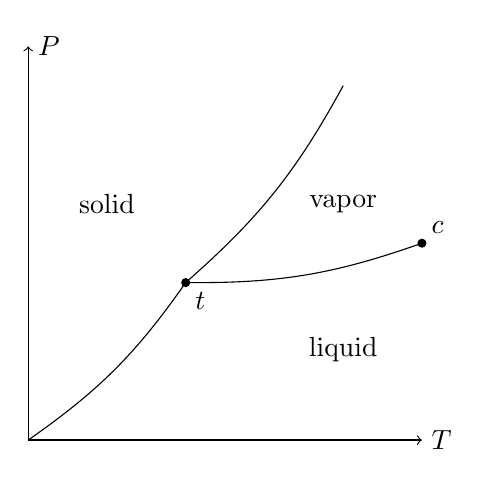
\begin{tikzpicture}
        \draw[->] (0,0) -- (5,0) node[right] {$T$};
        \draw[->] (0,0) -- (0,5) node[right] {$P$};
                
        \draw[] (0,0) to[bend right=10] (2,2) node[xshift=-1cm, yshift=1cm] {solid};
        \draw[] (2,2) to[bend right=10] (5,2.5) node[yshift=-1.35cm, xshift=-1cm] {liquid};
        \draw[] (2,2) to[bend right=10] (4,4.5) node[yshift=-1.5cm] {vapor};

        \filldraw[black] (2,2) circle (0.05) node[below right] {$t$};
        \filldraw[black] (5,2.5) circle (0.05) node[above right] {$c$};
        
        \end{tikzpicture}
        \caption{Qualitative phase diagram of the water. $t$ is a triple point and $c$ is a critical point.}
        \label{fig:phwater}
    \end{figure}

    \begin{figure}[h!]
        \centering
        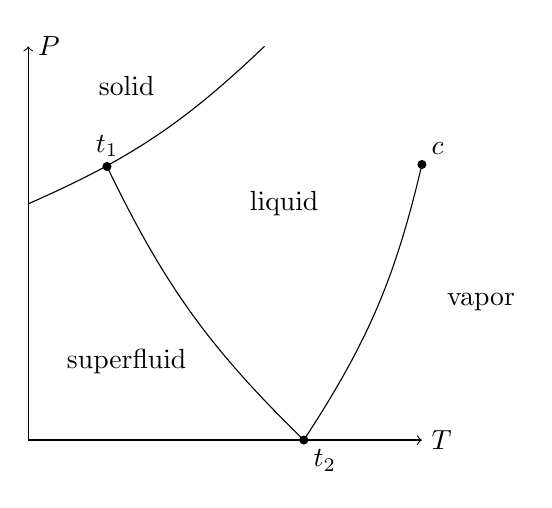
\begin{tikzpicture}
        \draw[->] (0,0) -- (5,0) node[right] {$T$};
        \draw[->] (0,0) -- (0,5) node[right] {$P$};
                
        \draw[] (0,3) to[bend right=10] (3,5) node[xshift=-1.75cm, yshift=-0.5cm] {solid};
        \draw[] (1,3.475) to[bend right=10] (3.5,0) node[yshift=1cm, xshift=-2.25cm] {superfluid};
        \draw[] (3.5,0) to[bend right=10] (5,3.5) node[yshift=-0.5cm, xshift=-1.75cm] {liquid} node[yshift=-1.75cm, xshift=0.75cm] {vapor};

        \filldraw[black] (1,3.475) circle (0.05) node[above] {$t_1$};
        \filldraw[black] (3.5,0) circle (0.05) node[below right] {$t_2$};
        \filldraw[black] (5,3.5) circle (0.05) node[above right] {$c$};
        
        \end{tikzpicture}
        \caption{Qualitative phase diagram of the Helium. $t_1$ and $t_2$ are triple points and $c$ is a critical point.}
        \label{fig:phhelium}
    \end{figure} 

    A coexistence line is a line along which $2$ phases are in equilibrium. A coexistence point or triple point is a point in which $3$ phases are in equilibrium. Examples in the water phase diagram of coexistence lines are $S-L$, $L-V$ and $S-V$ separation lines, whereas there is only a single triple point. To study when coexistence phases system are in equilibrium, we exploit the grand canonical ensemble. For coexistence lines, in order to have equilibrium, we have
    \begin{equation*}
        T_1 = T_2 ~, \quad T_1 = T_2 ~, \quad p_1 = p_2 ~, \quad \mu_1 = \mu_2 ~,
    \end{equation*}
    which provide respectively thermal, mechanical and chemical equilibrium. Writing $\mu$ in terms of the other thermodynamic functions, we obtain a constraint 
    \begin{equation*}
        \mu_1(T,p) = \mu_2(T,p) ~,
    \end{equation*}
    which individuates a line in the $(T, p)$ plane. Similarly, for triple points, in order to have equilibrium, we have
    \begin{equation*}
        T_1 = T_2 = T_3 ~, \quad p_1 = p_2 = p_3 ~, \quad \mu_1 = \mu_2 = \mu_3 ~,
    \end{equation*}
    where we have denoted with $1,2,3$ different phases. Writing $\mu$ in terms of the other thermodynamic functions, we obtain $2$ constraint s
    \begin{equation*}
        \mu_1(T,p) = \mu_2(T,p) = \mu_3(T,p) ~,
    \end{equation*}
    which individuates a point in the $(T, p)$ plane.

    We can generalise this result with the Gibbs' phase rule, which states that, in a system with $l$ distinct species, the number of coexistence phases in equilibrium $r$ is bounded above by 
    \begin{equation*}
        r \leq l + 2 ~.
    \end{equation*} 
    In the water case, $l = 1$ and $r = 3$, so that at most we have indeed $3$ coexisting phases.

    Notice that the coexistence curve $L-V$ terminates at a critical point, in which there is no more distinction between liquid and vapor, because we can circumnavigate from right to go from one phase to the other.

\section{Classification of phase transitions}

    Away from a critical point, a phase transition involves latent heat $\Delta q$, since $T$ is constant, but thermal energy is used or released to change the phase. It can be estimated via the Clausius-Clapeyron equation
    \begin{equation}\label{ph:cceq}
        \dv{p}{T} = \frac{s_2 - s_1}{v_1 - v_2} = \frac{\Delta q}{T \Delta v}  ~.
    \end{equation}
    \begin{proof}
        In order to remain along the coexistence line, the constraint holds
        \begin{equation*}
            \mu_1(p, T) = \mu_2 (p, T) ~.
        \end{equation*}
        We differentiate it using the chain rule, keeping in mind that $p = p(T)$,
        \begin{equation*}
            \pdv{\mu_1}{T} \Big \vert_p + \dv{\mu_1}{p} \Big \vert_T \dv{p}{T} = \pdv{\mu_2}{T} \Big \vert_p + \dv{\mu_2}{p} \Big \vert_T \dv{p}{T} ~.
        \end{equation*}
        Hence, we isolate $dp/dT$ and we find
        \begin{equation*}
            \dv{p}{T} = \frac{\pdv{\mu_1}{T} \vert_p - \pdv{\mu_2}{T} \vert_p}{\pdv{\mu_2}{p} \vert_T - \pdv{\mu_2}{p} \vert_T} ~.
        \end{equation*}
        Since a change in phase does not mean a change in total number of particles, we can work with a fixed amount of them. The thermodynamic potential to use is therefore the Gibbs free energy $G(p, T, N) = \mu (p, T) N$ or the Gibbs free energy per particle 
        \begin{equation*}
            g = \frac{G}{N} = \mu(p,T) ~.
        \end{equation*}
        Using the last relation of~\eqref{td:es:g}
        \begin{equation*}
            \pdv{\mu}{p} \Big \vert_T = \pdv{g}{p} \Big \vert_T = \frac{1}{N} \pdv{G}{p} \Big \vert_T = \frac{V}{N} = v ~,
        \end{equation*}
        whereas, using the first relation of~\eqref{td:es:g}
        \begin{equation*}
            \pdv{\mu}{T} \Big \vert_p = \pdv{g}{T} \Big \vert_p = \frac{1}{N} \pdv{G}{T} \Big \vert_p = - \frac{S}{N} = - s ~.
        \end{equation*}
        Combining the $two$, we obtain
        \begin{equation*}
            \dv{p}{T} = \frac{\pdv{\mu_1}{T} \vert_p - \pdv{\mu_2}{T} \vert_p}{\pdv{\mu_2}{p} \vert_T - \pdv{\mu_2}{p} \vert_T} = - \frac{s_1 - s_2}{v_2 - v_1} = \frac{s_2 - s_1}{v_2 - v_1} ~.
        \end{equation*}
        Finally, using the second law of thermodynamics~\eqref{td:2nde}, we find
        \begin{equation*}
            \Delta s = \frac{\Delta q}{T} ~,
        \end{equation*}
        which implies that
        \begin{equation*}
            \dv{p}{T} = \frac{\Delta q}{T \Delta v} ~.
        \end{equation*}
    \end{proof}

    Suppose that in a system there is latent heat. Observing~\eqref{ph:cceq}, we can state that the latent heat $\Delta q$ is different from zero, only when $s_1 \neq s_2$, which corresponds to a change in order of the system. Recalling the first of~\eqref{td:es:g}, we can say that the phase $1$ must be more stable at low temperatures while phase $1$ must be more stable at high temperatures. This implies that there is a cusp-like behaviour of $G$, or equivalently on $\mu$,
    \begin{equation*}
        \pdv{\mu_1}{T} > \pdv{\mu_2}{T} ~.
    \end{equation*}
    Therefore, at the phase transition temperature, the Gibbs free energy is continuous ($\mu_1 = \mu_2$) but its first derivative in $T$ is not, resulting in a cusp-like behaviour. Moreover, if it does change volume as well $v_2 \neq v_1$, its first derivative in $p$ has a similar behaviour. However, at $T = T_c$, discontinuity of first derivatives disappears, since we cannot distinguish anymore the $2$ phases. However, there could be other discontinuities in higher derivatives, e.g.~specific heat or compressibility are defined as second derivatives of thermodynamic potentials. Hence, we classify phase transitions in $2$ different kind 
    \begin{enumerate}
        \item $1$st order phase transitions, i.e.~those in which the $1$st derivatives of thermodynamic potentials are discontinuous;
        \item continuous phase transitions, i.e.~those in which the higher derivatives of thermodynamic potentials are discontinuous.
    \end{enumerate}
    In our case, the former are those in which there is a jump $v_2 \neq v_1$ and $s_2 \neq s_1$ and the latter are those in which $v_2 = v_1$ and $s_2 = s_1$. To summarise, a phase transition happens when there is a singular point for a thermodynamic potential.  
    In the next section, we will develop the mathematical framework of a phase transition in terms of this quantity in the thermodynamic limit.

\section{Theorems of Lee and Young}

    Consider a classical fluid in a volume $V \subset \mathbb R^3$. As mentioned before, we will analyse it in the grand canonical ensemble. The Hamiltonian of the system is 
    \begin{equation*}
        H = \sum_{i=1}^{N} (\frac{p_i^2}{2m} + U_N (q_i)) 
    \end{equation*}
    and the grand canonical partition function is 
    \begin{equation*}
        \mathcal Z (z, T, V) = \sum_{N=0}^\infty z^N \frac{Q_N (T, V)}{N! \lambda_T^3} ~,
    \end{equation*}
    where we have defined a positive quantity
    \begin{equation*}
        Q_N (T, V) = \int_{V^N} \prod_{i=1}^N d^3 q^i \exp (- \beta U_N(q^i)) ~.
    \end{equation*}
    \begin{proof}
        The canonical partition function~\eqref{c:z} is
        \begin{equation*}
        \begin{aligned}
            Z_N & = \int_{\mathcal M^N} \prod_{i=1}^N \frac{d^3 q^i ~ d^3 p^i}{N! h^{3N}}\exp (- \beta \sum_j \frac{p_j}{2m} + U_N(q^i) ) \\ & = \frac{1}{N!} \underbrace{\int_{\mathbb R^{3N}} \prod_{i=1}^N \frac{d^3 p^i}{h^{3N}} ~ \exp(- \beta \frac{p_i}{2m})}_{\frac{1}{\lambda_T^{3N}}} \underbrace{\int_{V^N} \prod_{i=1}^N d^3 q^i ~\exp(-\beta U_N(q_i))}_{Q_N} = \frac{Q_N(T, V)}{N! \lambda_T^{3N}} ~.
        \end{aligned}
        \end{equation*}
        Finally, using ~\eqref{gc:z}, we find 
        \begin{equation*}
            \mathcal Z = \sum_{N=0}^\infty z^N Z_N = \sum_{N=0}^\infty z^n \frac{Q_N}{N! \lambda_T^{3N}} ~.
        \end{equation*}
    \end{proof}
    Now, we need to study when this power series in $z$ converges. The first step is to promote $z$ into a complex variable, but always keeping in mind that the physical states are only the ones for which $z \in \mathbb R^+$. A reasonable assumption for the behaviour of the potential is that $U_N$ is bounded from below by a constant that does not grow faster than $N$, i.e. $U_N \geq - BN$ with $B > 0$. This implies that 
    \begin{equation*}
        |\mathcal Z| \leq \exp(\frac{V \exp(\beta B) |z|}{\lambda_T^3}) ~.
    \end{equation*}
    \begin{proof}
        In fact, using the assumption, we have
        \begin{equation*}
            \exp(- \beta U_N) \leq \exp(\beta B N) ~,
        \end{equation*}
        hence, $Q_N$ becomes
        \begin{equation*}
            Q_N = \int_{V^N} \prod_{i=1}^N d^3 q^i \exp (- \beta U_N(q^i)) \leq \exp(\beta B N) \underbrace{\int_{V^N}\prod_{i=1}^N d^3 q^i}_{V^N} = \exp(\beta B N) V^N 
        \end{equation*}
        and the canonical partition function becomes
        \begin{equation*}
            Z_N = \frac{Q_N}{N! \lambda_T^{3N}} \leq \frac{V^N}{N! \lambda^{3N}_T} \exp(\beta B N) ~.
        \end{equation*}
        Finally, we find that the grand canonical partition function becomes
        \begin{equation*}
            |\mathcal Z| \leq \sum_{N=0}^\infty \frac{|z|^N}{N! \lambda_T^{3N}} V^N \exp(\beta B N) = \exp(\frac{V \exp(\beta B) |z|}{\lambda_T^3}) ~.
        \end{equation*}
    \end{proof}
    Notice that there is a problem. An exponential has an infinite convergence radius and, therefore, $\mathcal Z$ is analytical $\forall z \in \mathbb C$, in particular for $z \in \mathbb R^+$. Furthermore, $\mathcal Z$ cannot vanish $\forall N$ since it is convergent and it is a sum of positive terms. 

    Since we are working in the grand canonical ensemble, we can introduce a redefined grand potential
    \begin{equation*}
        \psi = \frac{\beta \Omega}{V} = \lim_{td} \frac{\ln \mathcal Z}{V} ~,
    \end{equation*}
    for which it is valid 
    \begin{equation*}
        p \beta = \psi ~, \quad n = z \pdv{}{z} \psi ~.
    \end{equation*}
    \begin{proof}
        For the first, using the first of~\eqref{gc:es}
        \begin{equation*}
            \Omega = - p V = - \frac{1}{\beta} \ln \mathcal Z ~,
        \end{equation*}
        hence
        \begin{equation*}
            p \beta = \frac{\ln \mathcal Z}{V} = \psi ~.
        \end{equation*}
        For the second, using the second of~\eqref{gc:es}
        \begin{equation*}
            N = z \pdv{}{z} \ln \mathcal Z = - \frac{z}{\beta} \pdv{}{z} \ln \Omega ~,
        \end{equation*}
        hence
        \begin{equation*}
            n = \frac{N}{V} = - \frac{z}{\beta} \pdv{}{z} \frac{\ln \Omega}{V} =  - \frac{z}{\beta} \pdv{}{z} \psi ~.
        \end{equation*}
    \end{proof}
    These results can be formally stated by $2$ theorems, proved by Lee and Young, in terms of $\psi$.
    \begin{theorem}[Lee, Young I]
        Let $U_N$ be the potential such that $U_N \geq - BN$ with $B > 0$. Let also that boundaries of the volume do not increase faster than $V^{2/3}$, in order to neglect surface terms. Then $\psi$ exists, it is a continuous and monotonically increasing function of $z \in \mathbb R^+$.
    \end{theorem}
    \begin{theorem}[Lee, Young II]
        Given an open subset of the complex plane containing an interval of $\mathbb R^+$ such that it does not contain zeroes of $\mathcal Z$, then $V^{-1} \ln \mathcal Z$ converges uniformly for $V \rightarrow \infty$ in any closed set of this region, $\psi$ exists and it is analytic.
    \end{theorem}
    This means that there are no phase transitions and there is a single stable phase, since there cannot happen singularities for zero-free regions. How is it possible? We have not yet computed the thermodynamic limit. In fact, consider a system composed by hard spheres occupying a finite volume $v$. Since particles cannot overlap, the maximum number of particles is $M = V / v$. Therefore, $\mathcal Z$ is a polynomial function in $z$ of degree $M$ and, by the fundamental theorem of algebra, it has exactly $M$ zeroes but, by the theorems of Lee and Young, no zeros are in $\mathbb R^+$. However, if we go into the thermodynamic limit ($V \rightarrow \infty$ implies that $M \rightarrow \infty$), the number of zeroes increases. It may happen that, at a certain temperature, zeroes accumulate towards an isolated point $z = z_c$, which divides $\mathbb R^+$ into $2$ regions corresponding $2$ different phases. $\mathcal Z (V \rightarrow \infty, T, \mu)$ has a zero in $z = z_c$. Furthermore, $\psi$ is continuous but it is not analytic anymore: $1st$ order phase transitions or continuous phase transitions may occur. See Figure~\ref{fig:accu}.
    
    \begin{figure}[h!]
        \centering
        \begin{tikzpicture}
        \draw[->] (-0.5,0) -- (4,0) node[right] {$\real z$};
        \draw[->] (0,-2) -- (0,2) node[right] {$\imm z$};
                
        \filldraw[black] (1.5, 1) circle (0.05) ;
        \filldraw[black] (1.75, 0.75) circle (0.05) ;
        \filldraw[black] (1.85, 0.5) circle (0.05) ;
        \filldraw[black] (1.95, 0.25) circle (0.05) ;
        \filldraw[black] (1.975, 0.1) circle (0.05) ;
        \filldraw[black] (2, 0) circle (0.05) node[above right] {$z_c$} node[yshift=-0.4cm, xshift=1.1cm] {phase 2} node[yshift=-0.4cm, xshift=-1.1cm] {phase 1};
        \filldraw[black] (1.975, -0.1) circle (0.05) ;
        \filldraw[black] (1.95, -0.25) circle (0.05) ;
        \filldraw[black] (1.85, -0.5) circle (0.05) ;
        \filldraw[black] (1.75, -0.75) circle (0.05) ;
        \filldraw[black] (1.5, -1) circle (0.05) ;
        
        \end{tikzpicture}
        \caption{Accumulation of zeros in $z = z_c$ in the complex plane of $z$ that divides the real axis into two different phases $1$ and $2$.}
        \label{fig:accu}
    \end{figure}

    In the next chapter, we will study the paradigmatic example for phase transitions: the Ising model.

\chapter{Ising model}

    The Ising model deals with spin. However, spin is a quantum physical quantity that does not have a classical counterpart, so when we talk about classical spin, we mean localised magnetic moments that couple with an external magnetic field. 

\section{Simple Ising model}
    
    Consider a system composed by a discrete lattice, e.g.~an hypercubic lattice in Figure~\eqref{fig:latt}, of dimension $d$. Lattice sites are labelled by $i \in \mathbb Z_d$. For each vertex,  there is a degree of freedom (classical spin) attached to a vector $\mathbf S_i \in \mathbf R^n$ with fixed magnitude $|\mathbf S_i| = $ const. Therefore, $\mathbf S_i \in \mathbb S^{n-1}$, where $\mathbb S^{n-1}$ is the $(n-1)$-dimensional sphere of radius $|\mathbf S_i|$. Two adjacent vertices are called neighborhoods. Each site has therefore $z$ neighborhood, called the coordination number. For a $d$-dimensional hybercubic lattice, $z = 2 d$. 

    \begin{figure}[h!]
        \centering
        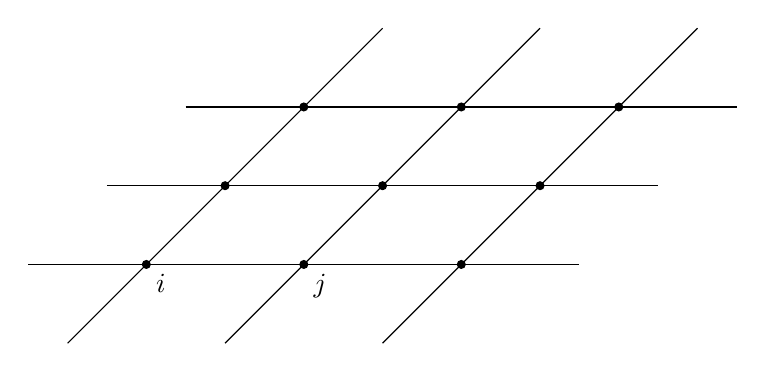
\begin{tikzpicture}
        \draw[-] (0,0) -- (4,4);
        \draw[-] (2,0) -- (6,4);
        \draw[-] (4,0) -- (8,4);
        \draw[-] (-0.5,1) -- (6.5,1);
        \draw[-] (0.5,2) -- (7.5,2);
        \draw[-] (1.5,3) -- (8.5,3);
                
        \filldraw[black] (1,1) circle (0.05) node[below right] {$i$};
        \filldraw[black] (3,1) circle (0.05) node[below right] {$j$};
        \filldraw[black] (5,1) circle (0.05) ;
        \filldraw[black] (2,2) circle (0.05) ;
        \filldraw[black] (4,2) circle (0.05) ;
        \filldraw[black] (6,2) circle (0.05) ;
        \filldraw[black] (3,3) circle (0.05) ;
        \filldraw[black] (5,3) circle (0.05) ;
        \filldraw[black] (7,3) circle (0.05) ;

        \end{tikzpicture}
        \caption{An hybercubic lattice of dimension $2$. $i$ and $j$ are neighbourhood sites}
        \label{fig:latt}
    \end{figure}

    We will not study the more general model, but we will restrict ourselves to the simple model in which $n = 1$ and the spin $\mathbf S_i$ can have only two values $\mathbf S_i = \sigma_i = \pm 1$. We will denote a possible configuration state as $\{\sigma_i\}_{i \in \mathcal L}$ and the phase space will be a discrete space composed by $2^N$ states $\{\{\sigma_i\}_{i \in \mathcal L} \colon \sigma_i = \pm 1\}$. The Hamiltonian of the system can be decomposed into two parts: a term that describes the interaction between neighborhood sites $H_{int}$ and a term that describes the coupling with an external field $H_{field}$ 
    \begin{equation*}
        H(\sigma_i) = H_{int} + H_{field} ~, \quad H_{int} = - J \sum_{i~\text{near}~j} \sigma_i \sigma_j ~, \quad H_{field} = - B \sum_{i=1}^{N} \sigma_i ~,
    \end{equation*}
    where $B$ is an external magnetic field and $J$ is the interaction constant, which is invariant under translations and rotations. We allow  sites to interact with each other because otherwise there would not have a phase transition.
    We can study what is the minimum energy configuration state according to the sign of $B$ and $J$:
    \begin{enumerate}
        \item for $J > 0$, all the spins are aligned $\sigma_i = \sigma_j$ for $i~\text{near}~j$, called ferromagnetic model;
        \item for $J < 0$, all the spins are antialigned $\sigma_i = - \sigma_j$ for $i~\text{near}~j$, called antiferromagnetic model;
        \item for $B > 0$, all the spins are aligned upwards $\sigma_i = + 1$;
        \item for $B < 0$, all the spins are aligned upwards $\sigma_i = - 1$. 
    \end{enumerate}
    Now, we will analyse the system in the canonical ensemble. Since we are in a discrete space, the canonical partition function is made over a sum of all the $2^N$ states, instead of an integral,
    \begin{equation*}
        Z_N = \sum_{\sigma_i = \pm 1} \exp(- \beta H(\sigma_i)) ~.
    \end{equation*}
    The thermodynamic equilibrium corresponds to the configuration of minimum (Helmoltz) free energy.

    Suppose the external magnetic field is shut down, i.e.~$B = 0$. What is the equilibrium configuration? At low temperature (and low energies), Helmoltz free energy is at minimum when entropy is small and all spins are aligned, because there are only $2$ possible states (all upwards or all downwards). At high temperature (and high energies), Helmoltz free energy is at minimum when entropy is large and all spins are random-aligned, because all spins point in all directions. 
    
    By means of the magnetisation
    \begin{equation}\label{ph:m}
        M = \av{\sum_{i=1}^N \sigma_i}_c = \sum_{i=1}^N \av{\sigma_i}_c ~,
    \end{equation}
    where the second expression follows from translation invariance, we can quantitatively study the phase transition.

\section{Mean-field approximation} 

    In general, it is difficult to compute the total canonical partition function because it cannot be reduced to the computation of the $1$-particle canonical partition function $Z_1$ since there is an interacting term
    \begin{equation*}
        Z_N = \sum_{\{\sigma_i = \pm 1\}} \exp(- \beta H) \neq (Z_1)^N ~.
    \end{equation*}
    However, we can make an useful approximation by neglecting the quadratic fluctuation term in the expansion of the interacting term in the Hamiltonian
    \begin{equation*}
    \begin{aligned}
        \sigma_i \sigma_j & = ((\sigma_i - m) + m)((\sigma_j - m) + m) \\ & = m^2 + m(\sigma_i - m) + m (\sigma_j - m) + (\sigma_i - m)(\sigma_j - m) \\ & \simeq m^2 + m(\sigma_i - m) + m (\sigma_j - m) \\ & = m^2 + m\sigma_i - m^2 + m \sigma_j - m^2 = - m^2 + m (\sigma_i + \sigma_j) ~,
    \end{aligned}
    \end{equation*}
    where $m = M / N$.
    The physical interpretation of the mean-field approximation is the following: when fluctuations with respect to the mean field $m$ are negligible, we do not have to compute every link with respect to each others but only with respect to the mean field $m$. In the mean-field approximation, the magnetisation is given by the equation 
    \begin{equation*}
        m = \tanh(\beta(Jzm + B)) ~.
    \end{equation*}
    \begin{proof}
        In fact, the Hamiltonian is 
        \begin{equation*}
        \begin{aligned}
            H_{mf} & = - J \sum_{i~\text{near}~j}  (- m^2 + m(\sigma_i + \sigma_j)) - B \sum_i \sigma_i \\ & = m^2 J \underbrace{\sum_{i~\text{near}~j} 1}_{\frac{Nz}{2}} - J m \sum_{i~\text{near}~j}  (\sigma_i + \sigma_j) - B \sum_i \sigma_i \\ & = \frac{m^2 z N J}{2} - Jmz \sum_i \sigma_i - B \sum_i \sigma_i = \frac{m^2 z N J}{2} - (J m z + B) \sum_i \sigma_i ~,
        \end{aligned}
        \end{equation*}
        where we have estimates that the number of links, given the coordination number $z$ which tells how many neighboring sites, is $Nz/2$.
        The canonical partition function becomes
        \begin{equation*}
        \begin{aligned}
            Z_N^{mf} & = \sum_{\{\sigma_i = \pm 1\}} \exp(- \beta H_{mf}) = \exp(- \beta \frac{J z n m^2}{2}) \sum_{\{\sigma_i = \pm 1\}} \exp(\beta (B + Jmz) \sum_i \sigma_i) \\ & = \exp(- \beta \frac{J z n m^2}{2}) (\sum_{\{\sigma_i = \pm 1\}} \exp(\beta (B + Jmx) \sigma_i))^N \\ & = \exp(- \beta \frac{J z n m^2}{2}) (\exp(\beta(B + Jmz)) + \exp(- \beta (B + Jmz)))^N \\ & = \exp(- \beta \frac{J z n m^2}{2}) (2 \cosh (\beta (B + Jmz)))^N ~.
        \end{aligned}
        \end{equation*}
        The Helmoltz free energy is 
        \begin{equation*}
        \begin{aligned}
            F & = - \frac{1}{\beta} \ln Z_N^{mf} = - \frac{1}{\beta} (- \beta \frac{J z N m^2}{2}) N \ln (2 \cosh (\beta (B + Jmz))) \\ & = \frac{J z N m^2}{2} N \ln (2 \cosh (\beta (B + Jmz))) ~.
        \end{aligned}
        \end{equation*}
        The magnetisation is 
        \begin{equation*}
        \begin{aligned}
             m & = \frac{1}{N} \av{\sum_i \sigma_i}_c = \frac{1}{N} \sum_{\{\sigma_i = \pm 1\}} \sum_i \sigma_i \exp(- \beta H) \\ & = - \frac{1}{\beta N} \sum_{\{\sigma_i = \pm 1\}} \frac{1}{Z_N} \pdv{}{\beta} \exp(- \beta H) = - \frac{1}{\beta N} \pdv{\ln Z_N}{\beta} ~.
        \end{aligned}
        \end{equation*}
        Hence 
        \begin{equation*}
            m = \tanh (\beta (B + J m z)) ~.
        \end{equation*}
    \end{proof}
    
    Now, we have a self-consistent equation for $m$ to solve. The condition for having a solution is 
    \begin{equation}\label{ph:m1}
        m \begin{cases}
            > 0 & B > 0 \\
            < 0 & B < 0 \\
        \end{cases} ~.
    \end{equation}
    Particular attention is the study of the solution for $B = 0$. The magnetisation becomes
    \begin{equation*}
        m = \tanh \frac{J m z}{k_B T} = \tanh (\frac{T_c}{T} m) ~,
    \end{equation*}
    where $T_c = J z / k_B$ is the critical temperature, that depends on $z$. Calling $\tilde m = T_c m / T$, we have 
    \begin{equation*}
        \frac{T \tilde m}{T_c} = \tanh \tilde m ~,
    \end{equation*}
    which can be solved graphically by finding the intersection between the plots of the right-handed side (a straight line) and of the left-handed side (an hyperbolic tangent).See Figure~\ref{mf:m}.
    \begin{figure}[h!]
        \centering
        \scalebox{0.7}{\pyc{plot4('x', '2* x', 'x / 2', 'x', 'tanh(x)', 5, 5, 20, True, False, False)}}
        \caption{A plot of the graphical solution of $T \tilde m / T_c = \tanh \tilde m$ for different value of $T/T_c = 1/2, 1, 2$.}
        \label{mf:m}
    \end{figure}
    Therefore, by looking at the plot, we can conclude that 
    \begin{enumerate}
        \item for $T \geq T_c$, there is only one solution $m = 0$;
        \item for $T < T_c$, there are two non-trivial solutions $m(T) = \pm m_0 (T)$, one positive and one negative.
    \end{enumerate}
    To summarise 
    \begin{equation}\label{ph:mtc}
        m = \begin{cases}
            0 & T > T_c \\ 
            \pm m_0(T) & T < T_c \\ 
        \end{cases} ~.
    \end{equation}

    Now, we are able to compute the phase diagram $(T, B)$. In fact, for $B \neq 0$, we recover~\eqref{ph:m1}, whereas for $B=0$, $m \neq 0$ for $T < T_c$ (ferromagnetic phase) and $m = 0$ for $T \geq T_c$ (paramagnetic phase). See Figure~\eqref{fig:mtrans}. By looking at it, we can observe that $m$ is an order parameter, since when it is zero there is disorder and when it is different from zero, there is order. It signals as well when there is a phase transition, since by its value we can say if we are in a ferromagnetic or in a paramagnetic phase. See Figure~\eqref{fig:mt}.
    
    \begin{figure}[h!]
        \centering
        \begin{tikzpicture}
        \draw[->] (-0.5,0) -- (5,0) node[right] {$T$};
        \draw[->] (0,-2.5) -- (0,2.5) node[right] {$B$};
                
        \draw[thick] (0,0) -- (2.5,0) node[xshift=-1cm, yshift=0.25cm] {$m \neq 0$} node[xshift=1cm, yshift=0.25cm] {$m = 0$} node[xshift=-1cm, yshift=1.5cm] {$m > 0$} node[xshift=-1cm, yshift=-1.5cm] {$m < 0$};

        \filldraw[black] (2.5,0) circle (0.05) node[below right] {$T_c$};
        
        \end{tikzpicture}
        \caption{Phase diagram of the Ising model.}
        \label{fig:mtrans}
    \end{figure}
    
    \begin{figure}[h!]
        \centering
        \begin{tikzpicture}
        \draw[->] (-0.5,0) -- (5,0) node[right] {$T$};
        \draw[->] (0,-2.5) -- (0,2.5) node[right] {$M$};
                
        \draw[thick] (0,1.5) to[bend left=50] (2.5,0);
        \draw[thick] (0,-1.5) to[bend right=50] (2.5,0);
        \draw[thick] (2.5,0) -- (5,0);

        \filldraw[black] (2.5,0) circle (0.05) node[below right] {$T_c$};
        
        \end{tikzpicture}
        \caption{Qualitative plot of $M$ in function of $T$.}
        \label{fig:mt}
    \end{figure}

    In particular, in a neighborhood of $T_c$, we can estimate that the behaviour is
    \begin{equation}\label{ph:beta}
        M \sim (T - T_c)^\beta ~,
    \end{equation}
    where $\beta \in \mathbb R$ is a parameter and $T < T_C$. $beta$ characterises the phase transition, since it tells at which speed $M \rightarrow 0$ when approaching $T \rightarrow T_c$. It is one of the $6$ so-called critical exponents.

    Other information can be found in the $2$-point correlation function between $2$ different sites
    \begin{equation*}
        G_{ij} = \av{\sigma_i \sigma_j} - \av{\sigma_i} \av{\sigma_j} =  \av{\sigma_i \sigma_j} - m^2 ~,
    \end{equation*}
    which in the limit for which $r = |i - j|$ is large, it can be estimated to be 
    \begin{equation}\label{ph:eta}
        G(r) \propto \begin{cases}
            \exp(- \frac{r}{\xi}) & T \neq T_c \\
            r^{-d+2-\eta} & T = T_c \\
        \end{cases} ~,
    \end{equation}
    where $\xi$ is the correlation length 
    \begin{equation}\label{ph:nu}
        \xi(T) = |1 - \frac{T}{T_c}|^{-\nu} \xrightarrow{T \rightarrow T_c} \infty ~.
    \end{equation}
    where $\eta$ and $\nu$ are critical exponents. Physically, $\xi$ tells us what is the radius inside which all the spins are strongly correlated. For $ T = T_c$, all spins are correlated since they are all aligned. See Figure~\eqref{fig:phg}.

    \begin{figure}[h!]
        \centering
        \scalebox{0.7}{\pyc{plot1('x', 'exp(-x)', 3, 2, 21, True, True, True)}}
        \caption{A plot of the correlation function for $\xi = 1$ at $T \neq T_c$.}
        \label{fig:phg}
    \end{figure}

\section{Spontaneous symmetry breaking}

    In the classical fluid system, we can find phase transition by studying symmetries of the system. In fact, we can distinguish solid from fluid by the translation or rotations invariance, since solid has only discrete invariance, whereas fluid has continuous invariance. However, we cannot distinguish with symmetries between gas and liquid. This means that the phase transition $V-L$ is not breaking any symmetry, but the phase transition $L-S$ does. 
    Also in the Ising model, we can similarly notice that a phase transition can arise from a spontaneous symmetry breaking. In fact, the interacting term in the Hamiltonian $H_{int}$ is invariant under the global symmetry group $\mathbb Z_2$
    \begin{equation*}
        \sigma_i \rightarrow - \sigma_i ~, \quad \sigma_i \rightarrow \sigma_i ~.
    \end{equation*}
    However, the second term breaks explicitly the symmetry, since under this transformation it transforms as $H_{field} \rightarrow - H_{field}$. Moreover, notice that, by definition~\eqref{ph:m}, under this symmetry we have 
    \begin{equation}\label{ph:msymm}
        m = \frac{M}{N} = \frac{1}{N} \sum_{i=1}^N \av{\sigma_i}_c \rightarrow - \frac{1}{N}\sum_{i=1}^N \av{\sigma_i}_c = - \frac{M}{N} = - m ~,
    \end{equation} 
    which implies that the only possible value of $m$ is zero. In fact, for $T > T_c$ there is indeed $m=0$, but for $T < T_c$, the equilibrium state is no longer invariant under this symmetry. The Hamiltonian remains the same, but equilibrium states are not invariant anymore. This is the definition of a spontaneous symmetry breaking. 

    Formally, we can state that, at high temperature, we have a disordered phase, which is highly symmetric that correspond to a symmetry group $G$, whereas, at low temperature, we have an ordered phase, which is lowly symmetric that correspond to a symmetry subgroup $G_0 \subset G$. Let $O$ be an observable (not-invariant under $G$) such that 
    \begin{equation*}
        \phi = \av{O} = \begin{cases}
            0 & T > T_c \\
            \phi_0 (T) \neq 0 & T < T_c \\
        \end{cases} ~.
    \end{equation*}
    Then we say that a symmetry is spontaneously broken and $\phi$ is an ordered parameter. In the Ising model, we can identify $\phi = m$, since it is not invariant under $\mathbb Z_2$ by~\eqref{ph:msymm} and it is indeed a step function in $T = T_c$ by~\eqref{ph:mtc}.
    As phase transitions, also symmetry breaking needs the thermodynamic limit. In fact, we can arrive to a spontaneous symmetry breaking only in a way that are not equivalent. The first one is to shut down the external field and then compute the thermodynamic limit 
    \begin{equation*}
        \av{O}_{N, V, B \neq 0} \xrightarrow{B \rightarrow 0} 0 \xrightarrow{td} 0 ~.
    \end{equation*}
    The second one is to first compute the thermodynamic limit and then to shut down the external field 
    \begin{equation*}
        \av{O}_{N, V, B \neq 0} \xrightarrow{td} \av{O}_{n, B \neq 0} \xrightarrow{B \rightarrow 0} \begin{cases}
            0 & T > T_c \\
            O_0 \neq 0 & T < T_c \\
        \end{cases} ~.
    \end{equation*}
    Therefore, we can individuate $\phi$ as 
    \begin{equation*}
        \phi = \lim_{B \rightarrow 0} \lim_{td} \av{O}_{N, V, B} ~,
    \end{equation*}
    where the two limits do not commute.

\section{Critical exponents and universality classes}

    During the study of phase transitions, we some parameters like~\eqref{ph:beta},~\eqref{ph:eta} and~\eqref{ph:nu}. These are the critical exponents and they describe the behavior of physical quantities near the critical temperature of a phase transitions. We define the reduced temperature 
    \begin{equation*}
        \epsilon = \frac{T_c - T}{T_c} ~,
    \end{equation*}
    which tells us how much we are far away from the phase transition in terms of temperature. The critical exponent associated to an observable $f$ is 
    \begin{equation*}
        \lambda_f = \lim_{\epsilon \rightarrow 0} \frac{\ln f(\epsilon)}{\ln \epsilon} ~,
    \end{equation*}
    so that 
    \begin{equation*}
        f (\epsilon) \simeq g(\epsilon) |\epsilon|^{\lambda_f} ~.
    \end{equation*}
    \begin{proof}
        In fact, for $\epsilon \ll 1$,
        \begin{equation*}
            \frac{\ln f(\epsilon)}{\ln \epsilon} = \frac{\ln g(\epsilon) |\epsilon|^{\lambda_f}}{\ln \epsilon} = \underbrace{\frac{\ln g(\epsilon)}{\ln \epsilon}}_0 + \frac{\lambda_f \ln \epsilon}{\ln epsilon} \simeq \lambda_f ~.
        \end{equation*}
    \end{proof}
    
    The $6$ critical exponents are
    \begin{enumerate}
        \item $\alpha$ in the specific heat $C_{B = 0} \simeq |\epsilon|^{-\alpha}$,
        \item $\beta$ in the specific heat $\phi \simeq |\epsilon|^{\beta}$,
        \item $\gamma$ in the specific heat $\chi_{B = 0} \simeq |\epsilon|^{-\gamma}$,
        \item $\delta$ in the specific heat $B \simeq \sgn(\phi) |\phi|^{\delta}$,
        \item $\nu$ in the specific heat $\xi \simeq |\epsilon|^{-\nu}$,
        \item $\eta$ in the specific heat $G(r) \simeq r^{-d+2-\eta}$.
    \end{enumerate}
    $alpha$, $\gamma$ and $\nu$ have a minus sign to prevent divergences. They are calculated with the scaling hypothesis which states that Helmoltz free energy is an homogeneous function of $\epsilon$ and $B$ 
    \begin{equation*}
        f ( \lambda \epsilon, \lambda B) = \lambda f(\epsilon, B) ~.
    \end{equation*}

    Therefore, phase transitions can be classified into classes that are independent of the microscopic Hamiltonian. Due to the scale invariance, different systems may have the same behaviour of phase transition. The parameter of classification are 
    \begin{enumerate}
        \item dimension of the space $d$,
        \item symmetry group of the Hamiltonian $H$,
        \item residual symmetry subgroup $G_0$.
    \end{enumerate}
    Recall that the mean field approximation is exact for $d \geq 4$ while it works poorly for decreasing $d$. However, for $d = 2$, we have the exact solution.

